\documentclass{article}
\usepackage{arxiv}

\usepackage[utf8]{inputenc}
\usepackage[english, russian]{babel}
\usepackage[T1]{fontenc}
\usepackage{url}
\usepackage{booktabs}
\usepackage{amsfonts}
\usepackage{nicefrac}
\usepackage{microtype}
\usepackage{lipsum}
\usepackage{graphicx}
\usepackage{natbib}
\usepackage{doi}



\title{Differentiable algorithm for searching ensembles of deep learning models with diversity control}

\author{K. Yakovlev, O.Bakhteev, K. Petrushina, P. Babkin
	%% David S.~Hippocampus\thanks{Use footnote for providing further
	%%	information about author (webpage, alternative
	%%	address)---\emph{not} for acknowledging funding agencies.} \\
	%%Department of Computer Science\\
	%%Cranberry-Lemon University\\
	%%Pittsburgh, PA 15213 \\
	%%\texttt{hippo@cs.cranberry-lemon.edu} \\
	%% examples of more authors
	%%\And
	%%Elias D.~Striatum \\
	%%Department of Electrical Engineering\\
	%%Mount-Sheikh University\\
	%%Santa Narimana, Levand \\
	%%\texttt{stariate@ee.mount-sheikh.edu} \\
	%% \AND
	%% Coauthor \\
	%% Affiliation \\
	%% Address \\
	%% \texttt{email} \\
	%% \And
	%% Coauthor \\
	%% Affiliation \\
	%% Address \\
	%% \texttt{email} \\
	%% \And
	%% Coauthor \\
	%% Affiliation \\
	%% Address \\
	%% \texttt{email} \\
}
\date{}

\renewcommand{\shorttitle}{differentiable ensembles search}

%%% Add PDF metadata to help others organize their library
%%% Once the PDF is generated, you can check the metadata with
%%% $ pdfinfo template.pdf
\hypersetup{
pdftitle={Differentiable algorithm for searching ensembles of deep learning models with diversity control},
pdfsubject={q-bio.NC, q-bio.QM},
pdfauthor={K. Yakovlev, O.Bakhteev, K. Petrushina, P. Babkin},
pdfkeywords={First keyword, Second keyword, More},
}

\begin{document}
\maketitle

\begin{abstract}
	
This paper is developed to introduce a new method of creating ensembles of deep learning models. 
Many modern researches were focused on creating effective and efficient algorithms of differentiable architecture search,
missing oppotunity to create ensembles of deep learning models. This approach gives impressive results
as it was shown in few modern papers. In our research we investigate an algorithm of sampling deep learning models using
hypernetwork, which controls diversity of the models. This method allows us to sample deep learning models in one-shot,
withiout any additional calculational losses, this independence means that algorithm is able to sample as many models
as we want. To evaluate the performance of the proposed algorithm, we conducted experiments on the Fashion-MNIST and CIFAR-10
datasets and compare the resulting ensembles with ones sampled by other searching algorithms.

\end{abstract}


\keywords{ differential search \and neural emsembles \and hypernetwork \and diversity control }

\section{Introduction}

Nowadays algorithms of neural architecture search (NAS) are well-explored and prooved to be an effective way of creating
more effective and efficient neural networks. Such algorithms use different ways to make problem diffirentiable so it can
be solved by wide range of methods for smooth optimization problems. On the other hand, neural ensemble search (NES) is
modern and not as well investigated problem as NAS, although it is known that ensembles of deep learning models show better
results in different applied problems.

Our paper investigates an algorithm of sampling deep learning models in a new way. Despite the fact that similar algorithms
were discribed and investigated, our scheme has uniqeue set of techniques that gives compatible results and has its own sphere
of implimentations.

First of all, we use DARTS as our basic NAS algorithm. It is prooved to be an effective architecture search algorithm. Some
modern investigations have shown that the algorithm can be upgrated, but the modernisations do not make tangible difference
and are mainly made for some specific cases. So in our paper we are focusing on ensemble sampling, so slightly different base
model does not change anything in resulting ensemble.

Second of all, we use hypernetwork in our sampling algorithm. Hypernetwork is small network so it does not
consume too much computational capacity. This network contains information about another network, which is called target network.
This approach is not new: hypernetworks and supernetworks were intended to control different characteristics such as
complexity of acrhitecture or parameters of the target model in several modern investigations. In our algorithm it controls 
diversity of the target models, so every sampled model differs from previously sampled ones.

The hypernetwork uses Jensen-Shennon divergence (JSd) to measure difference between two architectures which is simmetric and finite
in contrast to more popular Kullback–Leibler divergence. Our main idea of sampling different model is to use a reguralizer,
based on JSd as a source of diversity.

This way we are able to sample deep learning models in one-shot, to sum up the scheme of our method:
\begin{enumerate} 
    \item find a base architectire using DARTS
    \item sample architectures in one-shot via differentiable algorithm
    \item inferencing answer is ensemble of the sampled deep learning models
\end{enumerate}


\section{Headings: first level}
\label{sec:headings}

\lipsum[4] See Section \ref{sec:headings}.

\subsection{Headings: second level}
\lipsum[5]
\begin{equation}
	\xi _{ij}(t)=P(x_{t}=i,x_{t+1}=j|y,v,w;\theta)= {\frac {\alpha _{i}(t)a^{w_t}_{ij}\beta _{j}(t+1)b^{v_{t+1}}_{j}(y_{t+1})}{\sum _{i=1}^{N} \sum _{j=1}^{N} \alpha _{i}(t)a^{w_t}_{ij}\beta _{j}(t+1)b^{v_{t+1}}_{j}(y_{t+1})}}
\end{equation}

\subsubsection{Headings: third level}
\lipsum[6]

\paragraph{Paragraph}
\lipsum[7]



\section{Examples of citations, figures, tables, references}
\label{sec:others}

\subsection{Citations}
Citations use \verb+natbib+. The documentation may be found at
\begin{center}
	\url{http://mirrors.ctan.org/macros/latex/contrib/natbib/natnotes.pdf}
\end{center}

Here is an example usage of the two main commands (\verb+citet+ and \verb+citep+): Some people thought a thing \citep{kour2014real, hadash2018estimate} but other people thought something else \citep{kour2014fast}. Many people have speculated that if we knew exactly why \citet{kour2014fast} thought this\dots

\subsection{Figures}
\lipsum[10]
See Figure \ref{fig:fig1}. Here is how you add footnotes. \footnote{Sample of the first footnote.}
\lipsum[11]

\begin{figure}
	\centering
	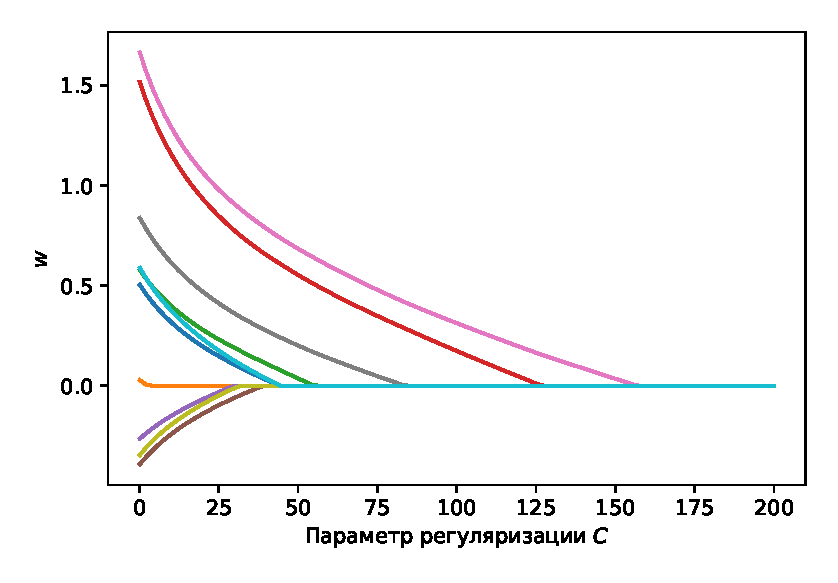
\includegraphics[width=0.5\textwidth]{../figures/log_reg_cs_exp.eps}
	\caption{Sample figure caption.}
	\label{fig:fig1}
\end{figure}

\subsection{Tables}
See awesome Table~\ref{tab:table}.

The documentation for \verb+booktabs+ (`Publication quality tables in LaTeX') is available from:
\begin{center}
	\url{https://www.ctan.org/pkg/booktabs}
\end{center}


\begin{table}
	\caption{Sample table title}
	\centering
	\begin{tabular}{lll}
		\toprule
		\multicolumn{2}{c}{Part}                   \\
		\cmidrule(r){1-2}
		Name     & Description     & Size ($\mu$m) \\
		\midrule
		Dendrite & Input terminal  & $\sim$100     \\
		Axon     & Output terminal & $\sim$10      \\
		Soma     & Cell body       & up to $10^6$  \\
		\bottomrule
	\end{tabular}
	\label{tab:table}
\end{table}

\subsection{Lists}
\begin{itemize}
	\item Lorem ipsum dolor sit amet
	\item consectetur adipiscing elit.
	\item Aliquam dignissim blandit est, in dictum tortor gravida eget. In ac rutrum magna.
\end{itemize}


\bibliographystyle{unsrtnat}
\bibliography{references}

\end{document}